\documentclass[conference]{IEEEtran}
\usepackage[english]{babel}
\usepackage[usenames,dvipsnames]{color}
\usepackage{amssymb}
\usepackage{amsmath}
\usepackage{cases}
\usepackage{url}
% \usepackage[mathscr]{euscript}
\usepackage{mathrsfs}
\usepackage{multirow}
\usepackage{booktabs}

\usepackage[maxnames=10, sorting=none]{biblatex}
\renewcommand*{\bibfont}{\scriptsize}

\makeatletter
\let\oldsection=\section
\newcommand{\oldsectionStar}[1]{\oldsection*{#1}}
\newcommand{\oldsectionStarless}[1]{\oldsection{#1}}
\renewcommand{\section}{\@ifstar\oldsectionStar\oldsectionStarless}

\let\oldsubsection=\subsection
\renewcommand{\subsection}[1]{\oldsubsection{#1}}
\makeatother

% ---- Text
\linespread{0.9}
\topmargin -60pt
\textheight 750pt

\definecolor{ipurple}{RGB}{195,0,191}
\newcommand{\note}[1]{{\color{ipurple}$\star$}\marginpar{\scriptsize\color{ipurple}#1}}

% ---- Tables
\setlength{\topsep}{0pt}
\setlength{\abovecaptionskip}{2pt}
\setlength{\belowcaptionskip}{0pt}

% ---- Formulas
\setlength\abovedisplayskip{5pt}
\setlength\belowdisplayskip{5pt}

% ---- References
\newcommand{\eref}[1]{Eq.~(\ref{equ:#1})}
\newcommand{\sref}[1]{Sec.~\ref{sec:#1}}
\newcommand{\tref}[1]{Tab.~\ref{tab:#1}}

\newcommand{\elabel}[1]{\label{equ:#1}}
\newcommand{\slabel}[1]{\label{sec:#1}}
\newcommand{\tlabel}[1]{\label{tab:#1}}

% Basic mathematics
\newcommand{\idot}{\cdot}
\newcommand{\eqdef}{\stackrel{\text{\tiny def}}{=}}
\newcommand{\ifrac}[2]{{{#1}/{#2}}}
\newcommand{\bigo}{\mathcal{O}}

% ---- Spaces
\renewcommand{\L}[1]{\mathcal{L}_{#1}}

% ---- Sets
\newcommand{\real}{\mathbb{R}}
\renewcommand{\natural}[1]{\mathbb{N}_{#1}}

% ---- Matrices
\newcommand{\mtx}[1]{(#1)}
\newcommand{\m}[1]{\mathbf{\MakeUppercase{#1}}}

\newcommand{\mI}{\m{I}}
\newcommand{\mZero}{\m{0}}

\newcommand{\diag}[1]{\text{diag}\left(#1\right)}

% ---- Vectors
\renewcommand{\vec}[1]{(#1)^T}
\let\vtick\v
\renewcommand{\v}[1]{\mathbf{#1}}

\newcommand{\vZero}{\v{0}}

% Probability theory
\newcommand{\outcomes}{\Omega}
\renewcommand{\o}{\omega}
\newcommand{\sAlgebra}{\mathscr{F}}
\newcommand{\pMeasure}{\mathscr{P}}

\newcommand{\rv}[1]{\MakeUppercase{#1}}
\newcommand{\mrv}[1]{\mathbf{\MakeUppercase{#1}}}

\renewcommand{\exp}{\mu}
\newcommand{\var}{\sigma^2}
\newcommand{\std}{\sigma}

\newcommand{\vExp}{{\boldsymbol\mu}}
\newcommand{\mCov}{\m{\Sigma}}

\newcommand{\oExp}[1]{\mathbb{E}\left[#1\right]}
\newcommand{\oVar}[1]{\mathbb{V}\text{ar}\left[#1\right]}
\newcommand{\oCov}[1]{\mathbb{C}\text{ov}\left[#1\right]}
\newcommand{\oCorr}[1]{\mathbb{C}\text{orr}\left[#1\right]}

\newcommand{\PDF}{\rho}

\renewcommand{\rv}{RV}
\newcommand{\rvs}{RVs}

% ---- Normal distribution
\newcommand{\normal}[2]{\mathcal{N}\left( #1, #2 \right)}

% Thermal model
\newcommand{\system}{\mathcal{S}}

% ---- Time
\renewcommand{\t}{t}
\newcommand{\dt}{\Delta \t}
\newcommand{\period}{\mathcal{T}}
\newcommand{\sTime}{\mathcal{T}}

% ---- Temperature
\newcommand{\T}{\Theta}
\newcommand{\vTI}{\v{\tilde{X}}} % Internal temperature
\newcommand{\vTO}{{\boldsymbol\Theta}} % Output temperature
\newcommand{\mTO}{{\boldsymbol\Theta}}

\newcommand{\amb}{\text{amb}}

% ---- Power
\newcommand{\vP}{\v{P}}
\newcommand{\mP}{\m{P}}

\newcommand{\dyn}{\text{dyn}}
\newcommand{\leak}{\text{leak}}

\newcommand{\f}{\mathcal{F}}

% ---- Capacitance and conductance
\newcommand{\mC}{\m{C}}
\newcommand{\mG}{\m{G}}

% ---- Processor elements/thermal nodes mapping
\newcommand{\mM}{\m{\tilde{B}}}

% ---- Profiles
\newcommand{\part}{\boldsymbol{\Delta}}
\newcommand{\prof}[1]{\Pi\left[\part, #1\right]}

% ---- Differential-algebraic system
% dx/dt = A * x + B * u
% y = B^T * x
\newcommand{\vX}{\v{X}}
\newcommand{\mA}{\m{A}}
\newcommand{\mB}{\m{B}}

\newcommand{\mE}{\m{E}}
\newcommand{\mD}{\m{D}}

% Polynomial Chaos
\newcommand{\support}{S}
\newcommand{\pcb}{\Phi}
\newcommand{\pcn}{\gamma}
\newcommand{\pcc}[1]{\hat{#1}}
\newcommand{\oPC}[3]{\mathcal{P}_{#1}^{#2}\left[#3\right]}

\makeatletter
\def\oInner#1{\@ifnextchar\bgroup{\oInnerDouble{#1}}{\oInnerSingle{#1}}}
\def\oInnerSingle#1{\left\langle #1 \right\rangle}
\def\oInnerDouble#1#2{\oInnerSingle{#1, #2}}
\makeatother

% ---- Integration
\newcommand{\qdn}[1]{\hat{#1}}
\newcommand{\qdw}{w}
\newcommand{\oQuad}[3]{\mathcal{Q}_{#1}^{#2}\left[#3\right]}

% Uncertain parameters
% ---- Correlated
\newcommand{\U}{U}
\newcommand{\vU}{\v{U}}

% ---- Independent
\newcommand{\Z}{Z}
\newcommand{\vZ}{\v{Z}}
\newcommand{\vz}{\boldsymbol{\zeta}}

\newcommand{\oTransform}[1]{T\left[#1\right]}
\newcommand{\oInvTransform}[1]{T^{-1}\left[#1\right]}

% ---- Process variation
\newcommand{\Leff}{L}
\newcommand{\nLeff}{L}
\newcommand{\gLeff}{{L^{(g)}}}
\newcommand{\lLeff}{L^{(l)}}
\newcommand{\Lth}{\lambda_\text{th}}
\newcommand{\corrLength}{\eta}

% Indexes
\newcommand{\nodes}{N_\text{n}}
\newcommand{\cores}{{N_\text{p}}}
\newcommand{\steps}{N_\text{s}}
\newcommand{\vars}{{N_\text{v}}}

\newcommand{\pcorder}{{N_\text{po}}}
\newcommand{\pcterms}{{N_\text{pt}}}

\newcommand{\qdlevel}{N_\text{ql}}
\newcommand{\qdorder}{N_\text{qo}}
\newcommand{\qdorderone}{\tilde{N}_\text{qo}}
\newcommand{\qdprecision}{N_\text{qp}}

\newcommand{\mcsamples}{N_\text{mcs}}

% Experimental results
\newcommand{\hostOS}{OS X 10.8}
\newcommand{\hostHardware}{a MacBook Pro 6.2 with Intel Core i7 2.66 GHz and 8 GB of RAM}
% \newcommand{\hostOS}{a GNU/Linux distribution}
% \newcommand{\hostHardware}{Intel Core i7 3.4 GHz with 8 GB of RAM}

\newcommand{\eExp}{\err{\mathbb{E}}}
\newcommand{\eVar}{\err{\mathbb{V}\text{ar}}}
\newcommand{\ePDF}{\err{\PDF}}

\newcommand{\err}[1]{\delta#1}

\newcommand{\mcs}[1]{\scriptstyle \mcsamples = 10^#1}
\newcommand{\csep}{\hspace{7pt}}
\newcommand{\psep}{\hspace{15pt}}


\begin{document}
  \title{Stochastic Temperature Analysis of\\Multiprocessor Systems}
  \author{Ivan Ukhov, Petru Eles, and Zebo Peng}

  \author{
    \IEEEauthorblockN{Ivan Ukhov}
    \IEEEauthorblockA{Link\"{o}ping University\\Sweden\\ivan.ukhov@liu.se}
    \and
    \IEEEauthorblockN{Petru Eles}
    \IEEEauthorblockA{Link\"{o}ping University\\Sweden\\petru.eles@liu.se}
    \and
    \IEEEauthorblockN{Zebo Peng}
    \IEEEauthorblockA{Link\"{o}ping University\\Sweden\\zebo.peng@liu.se}
  }

  \maketitle

  \begin{abstract}
    The stochastic temperature analysis (\sta) is important.
  \end{abstract}

  \section{Introduction and Prior Work} \slabel{introduction}
  The variations in the dynamic power due to the process variation are negligible whereas the leakage power is the major headache of the designer \cite{juan2012, srivastava2010}.

It is widely accepted that the leakage current has a log-normal distribution, cf. \cite{juan2012, srivastava2010}. The sub-threshold leakage is the most sensible to the process variation while the gate leakage has become less important with the introduction of high-k dielectrics \cite{juan2012}.

The most commonly used approach to perform the \sta\ is Monte Carlo sampling (MCS) techniques coupled with a deterministic thermal simulator. The problem is in the low rate of convergence, e.g., the mean value converges as $1/\sqrt{n}$ where $n$ is the number of simulations \cite{xiu2009}. Therefore, the MCS requires an unaffordably large number of realizations of the system to be performed.

In this work, we use a mathematical framework called the generalized polynomial chaos (gPC), which is the current state-of-the-art of numerical analysis of stochastic systems \cite{xiu2009, xiu2002}. The core of the gPC is the decomposition of stochastic processes into infinite sums of orthogonal polynomials of random variables (r.v.'s) that significantly eases the subsequent analysis. As its name suggests, the gPC is a generalization of the original polynomial chaos (PC) where only Hermite polynomials and Gaussian r.v.'s were considered \cite{ghanem1991}. In contrast, the gPC employs a broad family of orthogonal polynomials from the Askey scheme, which the Hermite polynomials are a subset of, and handles different probability distributions. It can be shown that \emph{any} functional with a finite variance can be approximated with a PC/gPC expansion, and this expansion converges in the $\L{2}$ (mean-square) sense.

In \cite{shen2009}, the PC is applied to estimate the full-chip leakage current.

The output of the proposed framework constitutes the stochastic power profile of the multiprocessor system and the corresponding stochastic temperature profile.

A possible way to speed up the analysis is to employ the model-order reduction (MOR) techniques \cite{benner2011}, which can dramatically decrease the number of state variables of the system. These techniques can be considered as a preprocessing step and, therefore, they are applicable to all the above-mentioned methods.

The rest of the paper is organazed as follows.


  \section{Preliminaries}
  \subsection{Conventional Notations}
Throughout this article, we use the following notations. $\real$ is the set of real number and $\natural{n}$ is the set of integers greater or equal to $n$. Boldface letters denote vectors and matrices, e.g., $\m{M} = \mtx{m_{ij}} \in \real^{n \times m}$ denotes a $n \times m$ real matrix, and $\v{V} = \vec{v_i} \in \real^n$ denotes and an $n$-dimensional real column vector. $\m{M}^T$ and $e^\m{M}$ are the transpose and matrix exponential of $\m{M}$, respectively. $\diag{m_i} \in \real^{n \times n}$ denotes a $n \times n$ diagonal matrix. $\mI_n$ is the $n \times n$ identity matrix, and $\mZ_{n \times m}$ is the $n \times m$ zero matrix; we shall omit these indexes when the actual dimensions of $\mI$ and $\mZ$ are clear from the context.

\subsection{Elements of Probability Theory}
Let $(\outcomes, \sAlgebra, \pMeasure)$ be a complete probability space \cite{durrett2010} where $\outcomes$ is a set of outcomes, $\sAlgebra \subset 2^\outcomes$ is a $\sigma$-algebra on $\outcomes$, and $\pMeasure: \sAlgebra \to [0, 1]$ is a probability measure induced on the measurable space $(\outcomes, \sAlgebra)$. A $\sAlgebra$-measurable function $\rv{X}(\o): \outcomes \to \real$ is called a \definition{random variable} (r.v.). Denote $\exp_\rv{X} = \oExp{\rv{X}(\o)}$ the expectation of $\rv{X}(\o)$ and $\var_\rv{X} = \oVar{\rv{X}(\o)}$ its variance. A $\pMeasure$-measurable, vector-valued function $\mrv{X}(\o): \outcomes \to \real^n$ is called a multivariate random variable (m.r.v.) with $\vExp_\mrv{X} = \oExp{\mrv{X}(\o)}$ and $\mCov_\mrv{X} = \oCov{\mrv{X}(\o)}$ being its expectation vector and covariance matrix, respectively. A \definition{stochastic process} is a parametrized collection of r.v.'s $\{ \rv{X}(\o, \t) \}_{\t \in \sTime}$ where $\sTime$ is a parameter space, which is usually assumed to be the real half line $[0, \infty)$ meaning time. $\{ \mrv{X}(\o, \t) \}_{\t \in \sTime}$ denotes a $n$-dimensional stochastic process. We shall omit the argument $\o \in \outcomes$ when the stochastic nature of the quantity under consideration is clear from the context.

The covariance matrix is necessarily a real, symmetric matrix. Therefore, it admits the eigenvalue factorization \cite{press2007} in the form $\mCov_\mrv{X} = \m{V}_{\mCov_\mrv{X}} \m{\Lambda}_{\mCov_\mrv{X}} \m{V}_{\mCov_\mrv{X}}^T$ where $\m{V}_{\mCov_\mrv{X}}$ and $\m{\Lambda}_{\mCov_\mrv{X}}$ are an orthogonal matrix of the eigenvectors and a diagonal matrix of the eigenvalues of $\mCov_\mrv{X}$, respectively. Denote $\oEigen{\mCov_\mrv{X}} = \m{V}_{\mCov_\mrv{X}} {\m{\Lambda}_{\mCov_\mrv{X}}}^\ifrac{1}{2}$. In this notation, $\mCov_\mrv{X} = \oEigen{\mCov_\mrv{X}} \oEigen{\mCov_\mrv{X}}^T$. Consequently, $\mrv{X}$ can be normalized as $\mrv{X} = \oEigen{\mCov_\mrv{X}} \mrv{y} + \vExp_\mrv{X}$ where $\oExp{\mrv{y}} = \mZ$ and $\oCov{\mrv{y}} = \mI$.

\subsection{Architecture Model} \slabel{architecture-model} \slabel{system-profiles}
Consider a multiprocessor platform that comprises $\cores$ processing elements of any kind and is equipped with a thermal package. Let $\system$ be a \definition{high-level description} of the platform that includes the following information:
\begin{itemize}
  \item The floorplan of the die (the location and dimensions of the processing elements). In the case of 3D ICs, the floorplans of each of the stacked chips.
  \item The configuration of the thermal package (the dimensions of each of the layers).
  \item The thermal parameters of the materials that the die and package are made of (the thermal conductivity, specific heat, convection capacitance, and convection resistance).
\end{itemize}

Suppose the given system depends on a number of \definition{uncertain parameters}, i.e., r.v.'s that are possibly correlated. Let $(\outcomes, \sAlgebra, \pMeasure)$ be the corresponding probability space and $\vU(\o) = \vec{\param_i(\o)} \in \real^\vars$, $\o \in \outcomes$, be a $\vars$-dimensional vector of these parameters. In this work, we assume that the uncertainties $\vU(\o)$, $\o \in \outcomes$, are a result of the process variation and manifest themselves in the deviation of the actual power dissipation of the system from the nominal value (see \sref{power-model}). In this case, $\outcomes$ represents the outcomes of the manufacturing process, which the given multiprocessor system is a product of. For brevity, we shall not write explicitly the dependency on $\vU(\o)$ and use $\o$ instead, i.e., $f(\o)$ should be understood as $f(\vU(\o))$.

Let $\prof{\m{Q}}$ be a \definition{system profile} of a quantity $Q$ over a time interval $\period$ where $\part = \{ 0 = \t_1 < \dotsc < \t_{\steps + 1} = \period \}$ is a partition of $\period$ into $\steps$ subintervals $\{ \dt_i = \t_{i+1} - \t_i \}_{i = 1}^{\steps}$, and $\m{Q} \in \real^{\cores \times \steps}$ is a matrix that captures the values of $Q$ for all $\cores$ processing elements at all $\steps$ time intervals. In particular, we are interested in the power and temperature profiles denoted by $\prof{\mP}$ and $\prof{\mTO}$, respectively (hereafter, $P$ stands for power and $\Theta$ for temperature). Since the system under consideration is affected by the process variation, we make a distinction between deterministic (nominal) or stochastic power and temperature profiles. In the stochastic case, each column of a system profiles is a m.r.v. with a known multivariate probability distribution.


  \section{Problem Formulation}
  The total dissipation of power is composed of two major parts: dynamic and static.
The influence of process variation on the dynamic power is known to be negligibly small \cite{srivastava2010}; on the other hand, the variability of the static power is substantial, in which the subthreshold leakage current contributes the most \cite{juan2011, juan2012}.
Hence, we shall focus on the subthreshold leakage and, more specifically, on the effective channel length, denoted by $\Leff$, since it has the strongest influence on leakage and is severely deteriorated by process variation \cite{chandrakasan2001}.
In particular, $\Leff$ also affects the threshold voltage \cite{juan2011}.

It is well known that the dispersion due to process variation of the effective channel length around the nominal value resembles a bell shape, which is similar to the ones owned by Gaussian distributions.
Therefore, such variations are often conveniently modeled using Gaussian variables \cite{srivastava2010, juan2011, juan2012, chandra2010, huang2009, lee2013, shen2009, bhardwaj2006, ghanta2006}.
In this work, due to both the underlying physics and demonstration purposes, we make a step further and bake right into the model the fact that the effective channel length---occupying the space between the drain and source of a nanoscopic transistor---cannot be arbitrarily large or take a negative value, as Gaussian distributions allow it to do.
In other words, we require the model of $\Leff$ to have a bounded support.
With this in mind, we propose to model physically-bounded parameters using the four-parametric family of beta distributions: $\dBeta(a, b, c, d)$ where $a$ and $b$ are the shape parameters, and $c$ and $d$ are the left and right bounds of the support, respectively.
$a$ and $b$ can be chosen in such a way that the typically found bell shape of the distribution is preserved.
An illustration is given in \fref{beta-normal} where we fitted a beta distribution to the standard Gaussian distribution.\footnote{Alternatively, one can match the moments of the distributions.}
It can be seen that the curves are nearly indistinguishable, but the beta one has a bounded support $[-4, 4]$, which can potentially lead to more realistic models.

\begin{figure}[t]
  \centering
  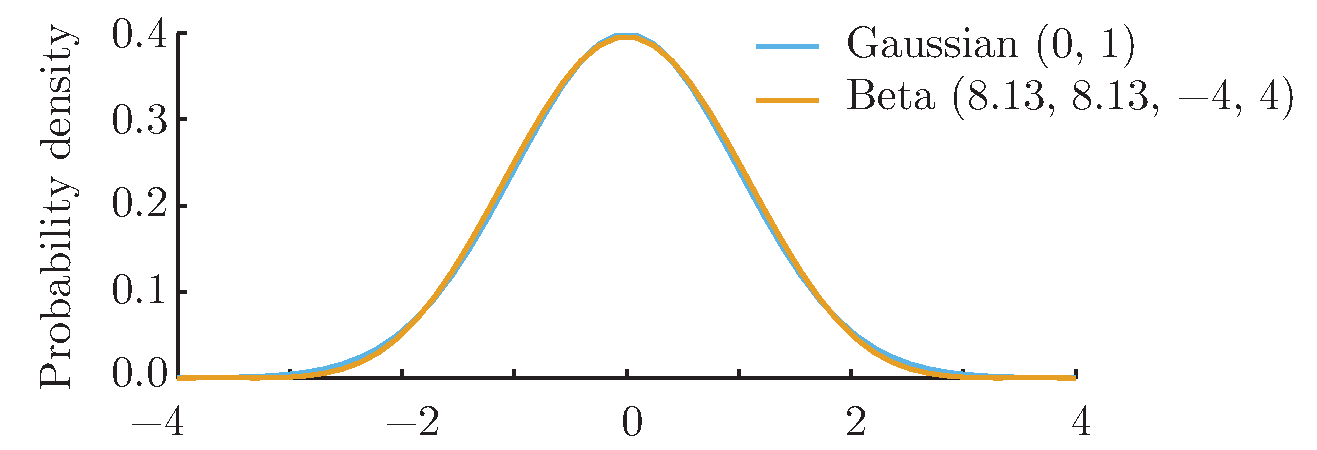
\includegraphics[width=0.9\ColumnWidth]{include/assets/beta-normal.pdf}
  \caption{The standard Gaussian distribution and a fitted beta distribution.}
  \flabel{beta-normal}
\end{figure}

The variability of $\Leff$ is split into global $\gLeff$ and local $\lLeff$ parts \cite{chandra2010, shen2009}.\footnote{Without loss of generality, $\gLeff$ can be treated as a composition of independent inter-lot, inter-wafer, and inter-die variations; likewise, $\lLeff$ can be treated as a composition of independent and dependent local variations.}
$\gLeff$ is assumed to be shared among all processing elements whereas each processing element has its own local parameter $\lLeff_i$.
Therefore, the effective channel length the $i$th processing element is modeled as follows:
\begin{equation} \elabel{leakage-partition}
  \Leff_i = \nLeff + \gLeff + \lLeff_i
\end{equation}
where $\nLeff$ is the nominal value of the effective channel length.
Hence, the uncertain parameters of the problem are
\begin{equation} \elabel{uncertain-parameters}
  \vU = \vec{\lLeff_1, \dotsc, \lLeff_\nprocs, \gLeff}.
\end{equation}

Global variations are typically assumed to be uncorrelated with respect to the local ones.
The latter, however, are known to have high spatial correlations, which we shall model using the following correlation function:
\begin{equation} \elabel{correlation-function}
  \fCorr(\vR_i, \vR_j) = \eta \; \fCorrSE(\vR_i, \vR_j) + (1 - \eta) \fCorrOU(\vR_i, \vR_j)
\end{equation}
where $\vR_i \in \real^2$ is the spatial location of the center of the $i$th processing element relative to the center of the die. The correlation function is a composition of two kernels:
\begin{align*}
  & \fCorrSE(\vR_i, \vR_j) = \exp\left(- \frac{\norm{\vR_i - \vR_j}^2}{\lCorrSE^2} \right) \text{ and} \\
  & \fCorrOU(\vR_i, \vR_j) = \exp\left(- \frac{\abs{\,\norm{\vR_i} - \norm{\vR_j}\,}}{\lCorrOU} \right),
\end{align*}
which are known as the squared-exponential and Ornstein-Uhlenbeck kernels, respectively.
$\eta \in [0, 1]$ is a weight coefficient balancing the kernels; $\lCorrSE$ and $\lCorrOU > 0$ are so-called length-scale parameters; and $\norm{\cdot}$ stands for the Euclidean distance.
The choice of the correlation function in \eref{correlation-function} is guided by the observations of the correlations induced by the fabrication process \cite{chandrakasan2001, friedberg2005, cheng2011}: $\fCorrSE$ imposes similarities between the spatial locations that are close to each other, and $\fCorrOU$ imposes similarities between the locations that are at the same distance from the center of the die (see also \cite{huang2009, ghanem1991, lee2013, bhardwaj2008, ghanta2006}).
The length-scale parameters $\lCorrSE$ and $\lCorrOU$ control the extend of these similarities, \ie, the range wherein the influence of one point on another is significant.

Although \eref{correlation-function} captures certain features inherent to the fabrication process, it is still an idealization.
In practice, it can be difficult to make a justifiable choice and tune such a formula, which is a prerequisite for the techniques in \sref{prior-work} based on the (continuous) KL decomposition.
A correlation matrix, on the other hand, can readily be estimated from measurements and, thus, is a more probable input to PTA.
Thus, we use \eref{correlation-function} with the only purpose of constructing a correlation matrix of $\{ \lLeff_i \}$.
For convenience, the resulting matrix is extended by one dimension to pack $\gLeff$ and $\{ \lLeff_i \}$ together.
In this case, the correlation matrix obtains one additional non-zero element on the diagonal.
Taking into account the variances of the variable, the final covariance matrix of the whole random vector $\vU$ (see \eref{uncertain-parameters}) is formed, which we denote by $\mCov_\vU$.

To conclude, an input to our analysis is the marginal distributions of the parameters $\vU$, which are beta distributions, and the corresponding covariance matrix $\mCov_\vU$.


  \section{System Model}
  \subsection{Power Model} \slabel{power-model}
Without loss of generality, we focus on the leakage power as it is motivated in \sref{introduction}. The power dissipation of the system with $\cores$ processing elements at time $\t$ is modeled as
\[
  \vP(\t, \vTO(\t, \o), \o) = \vP_\dyn(\t) + \vP_\leak(\vTO(\t, \o), \o)
\]
where $\vP_\dyn, \vP_\leak \in \real^\cores$ are the dynamic and leakage power, respectively, and $\vTO \in \real^\cores$ is temperature. The leakage power is modeled as a function of temperature due to the well-known, strong interdependency between them.

\subsection{Thermal Model} \slabel{thermal-model}
Given the system description $\system$, an equivalent thermal RC circuit with $\nodes$ \definition{thermal nodes} is constructed \cite{kreith2000}. The structure of the circuit depends on the intended level of details defining the accuracy of the final model.

The thermal behaviour of the circuit is modeled with the following system of differential-algebraic equations (DAEs) with the state-space dimension equal to $\nodes$:
\begin{align*}
  & \mC \frac{d\vTI(\t, \o)}{d\t} + \mG \vTI(\t, \o) = \mM \vP(\t, \vTO(\t, \o), \o) \\
  & \vTO(\t, \o) = \mM^T \vTI(\t, \o) + \vTO_\amb
\end{align*}
$\mC, \mG \in \real^{\nodes \times \nodes}$ are the matrices of the thermal capacitance and conductance, respectively. $\mC$ is a diagonal matrix with positive elements, and $\mG$ is a symmetric, positive-definite matrix. $\vTI \in \real^\nodes$ is the state vector of the system, which corresponds to the difference between the temperature of the thermal nodes and the ambient temperature. $\vP \in \real^\cores$ is the input vector of the power dissipation of the processing elements, and $\mM \in \real^{\nodes \times \cores}$ is its mapping matrix to the thermal nodes. $\vTO \in \real^\cores$ is the output vector of the system, which is the temperature of the processing elements. Finally, $\vTO_\amb \in \real^\cores$ is the vector of the ambient temperature, which, for clarity of presentation and without loss of generality, we model as a deterministic variable.

For convenience, we perform an auxiliary transformation of the original system proposed in \cite{ukhov2012}. Let $\vX = \mC^{1/2} \vTI$, $\mA = \mC^{1/2} \mG \mC^{1/2}$, and $\mB = \mC^{1/2} \mM$, then
\begin{align}
  & \frac{d\vX(\t, \o)}{d\t} = \mA \vX(\t, \o) + \mB \vP(\t, \vTO(\t, \o), \o) \elabel{fourier} \\
  & \vTO(\t, \o) = \mB^T \vX(\t, \o) + \vTO_\amb \nonumber
\end{align}
where $\vX$ is the new state vector. It can be seen that the coefficient matrix $\mA$ preserves the properties of $\mG$, i.e., it is symmetric and positive-definite.


  \section{Generalized Polynomial Chaos (gPC)}
  At \stage{4}, the independent \rvs, power model, and thermal model are fused together under the desired workload, $\profilePdyn$, to produce the corresponding stochastic power $\profileP{\o}$ and temperature $\profileT{\o}$ profiles. The obtained stochastic profiles are nothing more than two polynomials of $\Z_1(\o)$ and $\Z_2(\o)$ with time-dependent coefficients.

The construction of PC expansions is based on the Hermite basis (see \tref{askey}) as it was found to be optimal in situations involving Gaussian parameters \cite{xiu2010}.
A one-dimensional example of the basis is given in \fref{hermite} where the first six Hermite polynomials $\{ \pcb_i(\z) \}_{i = 1}^6$ are displayed.

In two dimensions, assuming a second-total-order PC expansion, the temperature at the $k$th moment of time is
\begin{align*}
  \vTO_k(\o) &= \pccs_{k1} + \pccs_{k2} \Z_1(\o) + \pccs_{k3} \Z_2(\o) + \pccs_{k4} \Z_1(\o) \Z_2(\o) \\
  & \qquad \qquad {} + \pccs_{k5} (\Z_1(\o)^2 - 1) + \pccs_{k6} (\Z_2(\o)^2 - 1)
\end{align*}
where $\pccs_{ki}$ are vectors with two elements corresponding to the two processors.

Once the basis has been chosen, we need to compute the corresponding coefficients, specifically, $\pcc{\vP}_i$ in \eref{pc-expansion}. As shown in \aref{polynomial-chaos}, the computation of $\pcc{\vP}_i$ involves multidimensional integration with respect to the \pdf\ of the \rvs\ $\vZ(\o)$.
In numerical analysis, this task is typically accomplished by virtue of a quadrature rule \cite{press2007}, which, loosely speaking, is a weighted summation over the integrand values computed at prescribed points. A natural choice of a quadrature rule when the weight function is a Gaussian \pdf\ is the Gauss-Hermite quadrature. Further details are given in \aref{gauss-quadrature}.

To summarize, we have completed four out of five stages of the proposed UQ framework depicted in \fref{algorithm}. The result is a light surrogate of the model in \eref{fourier-system}. At each moment of time, the surrogate is composed of two $\nprocs$-valued polynomials, one for power and one for temperature, that are defined in terms of $\nvars$ mutually independent \rvs; an example of such a polynomial is given in \eref{pc-k}. The constructed representation can be trivially analyzed to retrieve various statistics of the system in \eref{fourier-system}, and this is \stage{5}\ in \fref{algorithm}, which will be illustrated as a part of the next section.

\begin{figure}
  \centering
  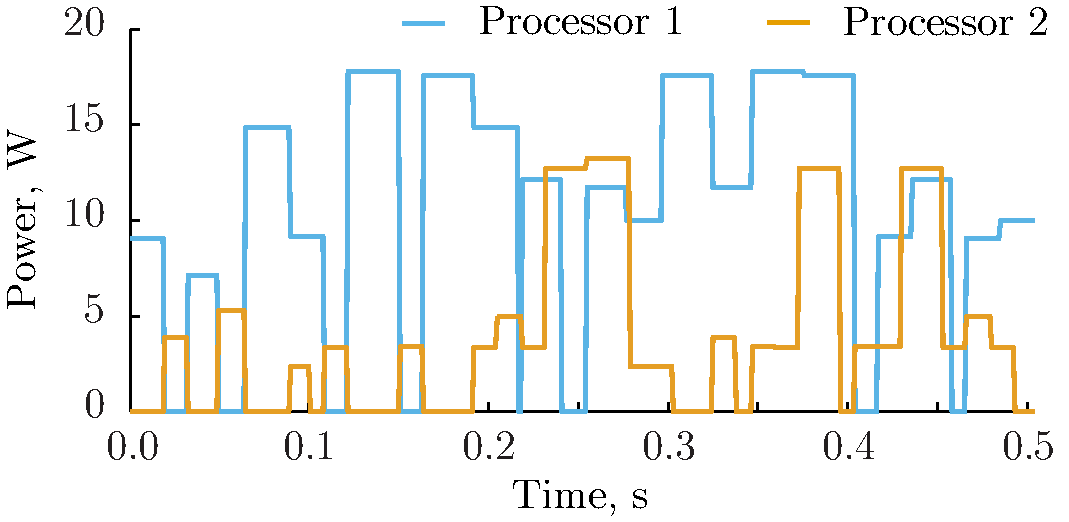
\includegraphics[width=1.00\columnwidth]{include/assets/application-power.pdf}
  \vspace{-0.5em}
  \caption{A dynamic power profile.}
  \flabel{application-power}
  \vspace{-0.5em}
\end{figure}

Assume that the dynamic power profile, $\profilePdyn$, corresponding to the considered workload is the one shown in \fref{application-power}.

\begin{figure}[bl]
  \vspace{-1.0em}
  \centering
  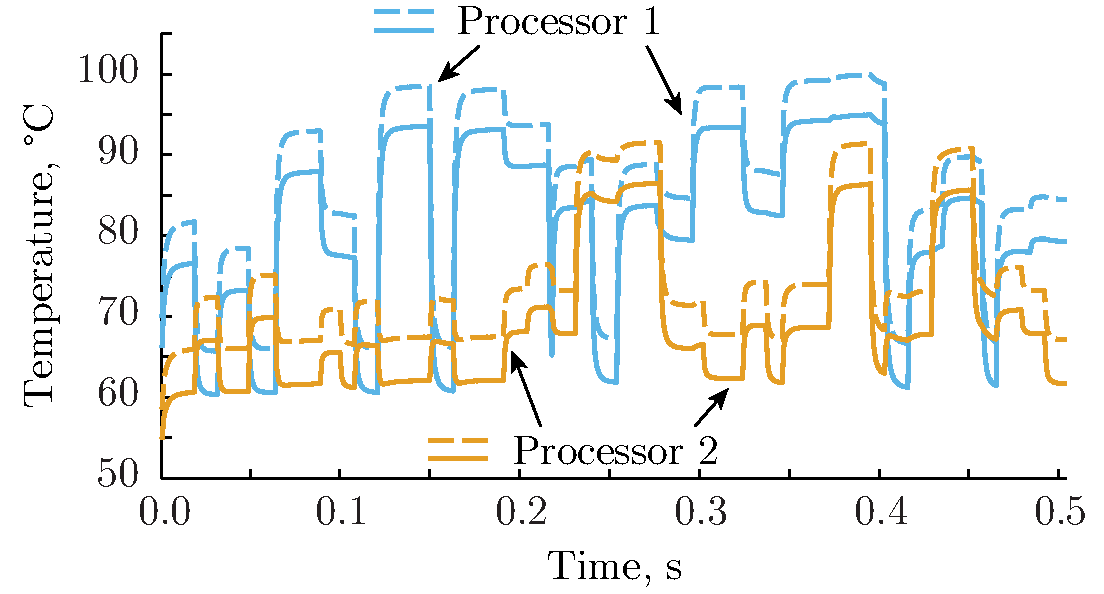
\includegraphics[width=0.90\columnwidth]{include/assets/application-temperature.pdf}
  \vspace{-0.5em}
  \caption{The expected temperature (the solid lines) and one standard deviation above it (the dashed lines).}
  \flabel{application-temperature}
\end{figure}

The expansion for power has the same structure but different coefficients.
Such a series might be shorter or longer depending on the accuracy requirements.
As we see, our surrogate model has a negligibly small computational cost to undertake UQ at \stage{5}: for any outcome of the uncertain parameters $\vZ(\o) \equiv \vZ$, we can easily compute the corresponding temperature by plugging $\vZ$ into the above equation; the same applies for power.
Thus, such characteristics as \cdfs\ and \pdfs\ (see \fref{motivation-pdf}) can be rigorously estimated. Furthermore, the expectation and variance at the $k$th moment of time are calculated as simply as
\[
  \oExp{\vTO_k(\o)} = \pccs_{k1} \hspace{1em} \text{and} \hspace{1em} \oVar{\vTO_k(\o)} = \sum_{i = 2}^{6} \pcn_i \: \pccs_{ki}^2
\]
where $\pcn_i$ are normalization constants, and the squaring should be understood element-wise.
For the nominal power profile $\profilePdyn$ depicted in \fref{application-power}, we obtain the corresponding stochastic temperature profile $\profileT{\o}$ and can observe, \eg, its expectation and standard deviation; they are plotted in \fref{application-temperature}.
The displayed curves closely match those obtained via MC simulations with $10^4$ samples; however, our method takes less than a second, on a personal laptop, while MC sampling takes more than a day, which we discuss in \sref{experimental-results}.


  \bibliographystyle{unsrt}
  \bibliography{include/references}
\end{document}
